\documentclass{article}
\usepackage[utf8]{inputenc}
\usepackage{amsmath}
\usepackage{listings}
\usepackage{graphicx}
\usepackage{hyperref}

\title{Bloom Filter}
\author{ Yannick Koller & Mike Gilgen }
\date{November 2022}

\begin{document}
    \maketitle

    \section{Einleitung}
    Ein Bloom Filter, benannt nach seinem Erfinder Burton Howard Bloom, ist eine auf Wahrscheinlichkeit basierende Set Datenstruktur. Anders als herkömmliche Set Datenstrukturen erlaubt der Bloom Filter kein entfernen von Elementen und liefert kein garantiertes Ergebniss für die Zugehörigkeit eines Elements. Dies erlaubt es einem Bloom Filter Speichereffizienter zu sein als herkömmliche Set Datenstrukturen.


    \section{Vor- und Nachteile}
    \begin{center}
        \begin{tabular}{c|c}
            Vorteil                & Nachteil                            \\
            \hline
            Effizient              & Fixe Grösse                         \\
            Keine false negatives  & Möglichkeit von false positives     \\
            Einfügen immer möglich & Kann überfüllen                     \\
            & Löschen von Elementen nicht möglich \\
        \end{tabular}
    \end{center}
    Die Möglichkeit von false positives ist sogenannten "Hash-Overlaps" geschuldet. Dabei kommt es bei nicht in der Menge vorhandenen Elementen zu den selben Hashwerten wie bei einem anderen, bereits in der Menge enthaltenem Element. Für alle gesuchten Elemente, die sich nicht in der Menge befinden, kann man dafür eine klare Aussage machen, dass sie nicht in der Menge ist. Daraus folgen zwei Aussagen die diese Datenstruktur zurückgibt wenn man die Zugehörigkeit eines Elements abfragt:

    \begin{itemize}
        \item Is probably in set (positive)
        \item Is definitely not in set (negative)
    \end{itemize}

    \clearpage


    \section{Praxisbeispiel}
    Der Webbrowser Google Chrome verwendete einen Bloom Filter um potenziell gefährliche URLs (wie z.B. Spam oder Malware) zu erkennen. Malwarescans werden auf Googles eigenen Servers gemacht was diese Operation Zeit- und Rechenaufwändig macht. Damit nicht jede Seite einem solchen Malwarescan unterzogen wird, wird zuerst der Bloom Filter befragt, ob eine URL potenziell gefährlich ist. Nur bei einem positiven Resultat wird die URL auf Googles eigenen Servern einem Malewarescan unterzogen.


    \section{Funktionsweise}
    Folgende Variablen werden für einen Bloom Filter benötigt:

    \begin{itemize}
        \item Erwartete Anzahl an Elementen $n$
        \item Gewünschte Fehlerquote $p$
        \item Anzahl benötigte Bits $m$
        \item Anzahl unterschiedliche Hashfunktionen $k$
    \end{itemize}

    Die optimalen Werte für Variablen $m$ und $k$ lassen sich aus $n$ und $p$ mit folgenden Formeln errechnen:

    \begin{equation}
        m = -\frac{n \ln{p}}{(\ln{2})^2}
    \end{equation}
    \begin{equation}
        k = \frac{m}{n} \ln{2}
    \end{equation}
    \begin{center}
        \textit{Die Herleitung der Formeln sind auf \href{https://en.wikipedia.org/wiki/Bloom_filter\#Optimal_number_of_hash_functions}{Wikipedia} auffindbar.}
    \end{center}
    Sind Variablen $m$ und $k$ bekannt, kann ein neuer, leerer Bloom Filter erstellt werden.
    \begin{center}
        \textit{pseudo Code}
    \end{center}
    \begin{lstlisting}
    // defining the Arrays
    HashFunctions[] hashFunctions;
    boolean[] filter;

    // defining the Hashalgorithms and build an empty filter
    boolean[] buildFilter(int n, double p){
        int m = (int) -((n * Math.log(p)) / (Math.log(2) * Math.log(2)));
        int k = (int) ((m / n) * Math.log(2));

        hashFunctions = new HashFunction[k];
        // feeding the filter
        for( int i = 0; i < k; i++ ) {
            hashFunctions[i] = Hashing.<hashAlogrithm>(RandomInt);
        }
        filter = new boolean[m] // empty filter
    }
    \end{lstlisting}
    Nun sind alle benötigten Komponenten des Bloom Filter verfügbar und der Filter lässt sich mit folgender Methode mit Elementen befüllen:
    \begin{center}
        \textit{pseudo Code}
    \end{center}
    \begin{lstlisting}
    void add(E element){
        for( HashFunction hashFunction : hashFunctions ){
            filter[hashFunction(element)] = true;
        }
    }
    \end{lstlisting}
    Die Abfrage, ob ein Element möglicherweise im Bloom Filter enthalten ist, funktioniert fast analog dem Einfügen:
    \begin{center}
        \textit{pseudo Code}
    \end{center}
    \begin{lstlisting}
    boolean mightContain(E element){
        for( HashFunction hashFunction : hashFunctions ){
            if( !filter[hashFunction(element)] ){
                return false;
            }
        }
        return true;
    }
    \end{lstlisting}
    Sobald an einer Stelle im Filter der Wert $false$ angetroffen wird, kann mit 100\% Sicherheit gesagt werden, dass ein Element nicht im Bloom Filter enthalten ist.

    \clearpage


    \section{Erkenntnisse aus unserem Projekt}
    Wir testen unseren Bloom Filter mit der erhaltenen Wörterliste. Dabei fügen wir nur die Hälfte aller Wörter in den Bloom Filter ein. Die erwartete False-Positive Wahrscheinlichkeit haben wir mit $p = 0,2$ initialisert.
    \\
    Mit der anderen Hälfte überprüfen wir die Korrektheit des Bloom Filters. Dabei zählen wir die False Positives und Vergleich deren Anteil im vergleich zur Totalanzahl an Wörtern. In unseren Versuchen variierte die Anzahl der False Positives zwischen 5600 und 5900 und die False Positives Rate schwankte um $0,2 \pm 0,01$ herum. Die False Positives Rate entspricht somit ziemlich genau der erwarteten Wahrscheinlichkeit von $p = 0,2$.
    \begin{figure}[h!]
        \centering
        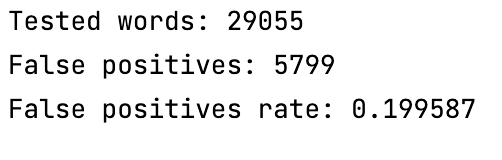
\includegraphics{./lib/dist_bloomResult.png}
        \caption{Bloom Result}
        \label{fig:Bloom Result}
    \end{figure}

\end{document}
